\chapter{Results and Discussion}

We used an established Rician smoothing method to combat noise in the diffusion images \cite{wiest2008rician}. This is a type of non-local smoothing technique which uses voxel to voxel similarity to guide the smoothing process. In general the parameters for this filtering method must be tuned to prevent oversmoothing, which can happen for instance if the weight is not sufficiently penalized when the similarity is not high enough. We used the publicly available MedInria software to carry out the filtering, and then to reconstruct the diffusion tensor from the raw diffusion weighted scans, from which fiber orientations were extracted as the first principal eigen vector. In practice we used a threshold on the FA map as a mask to restrict further processing.

\section{Qualitative Results}

\subsection{Importance of the filtering from the fibers...}

In topview figures \ref{fig:pig4_topviews} and a more transverse view where the helix angle is easier to visualize \ref{fig:pig4_helix}, we have a first glimpse at the difference of the fiber orientation and cohesion before and after smoothing the raw data through a Rician filter, which is the appropriate filtering method when dealing with DMRI data.\\
The region shown in figures \ref{fig:pig4_helix_no_smooth} and \ref{fig:pig4_helix_smooth} is a region away from the infarct where we should see a smooth turning of fibers. This region corresponds to the top-right region of the same slice presented in figures \ref{fig:pig4_topview_no_smooth} and \ref{fig:pig4_topview_smooth}.\\
Tracing fibers from raw data leads to an extremely noisy data from which it is hard to infer any general structure, which we will see in \ref{fig:histogram_pig6_no_smooth}. Indeed the low magnetic field value (1.5T) is one of the reasons why the data is not of the highest quality, as well as the low number of iterations in the acquisition process.\\
Thanks to the Rician smoothing it is again possible to guess the helix angle turning from outer wall to inner wall although this is still not perfect, as we want to keep as much information as possible with using the lightest filtering possible.

\begin{figure}
    \centering
    \begin{subfigure}{.48\textwidth}
        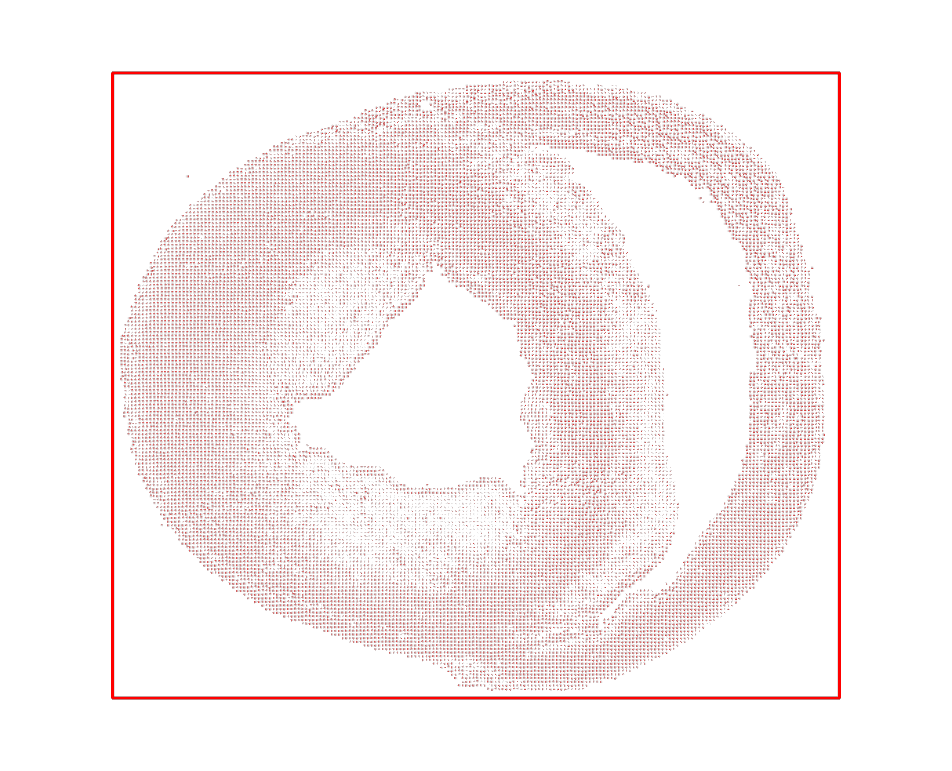
\includegraphics[width=\textwidth]{figures/pig4_topview_no_smooth}
        \caption{Without any smoothing}
        \label{fig:pig4_topview_no_smooth}
    \end{subfigure}
    \begin{subfigure}{.48\textwidth}
        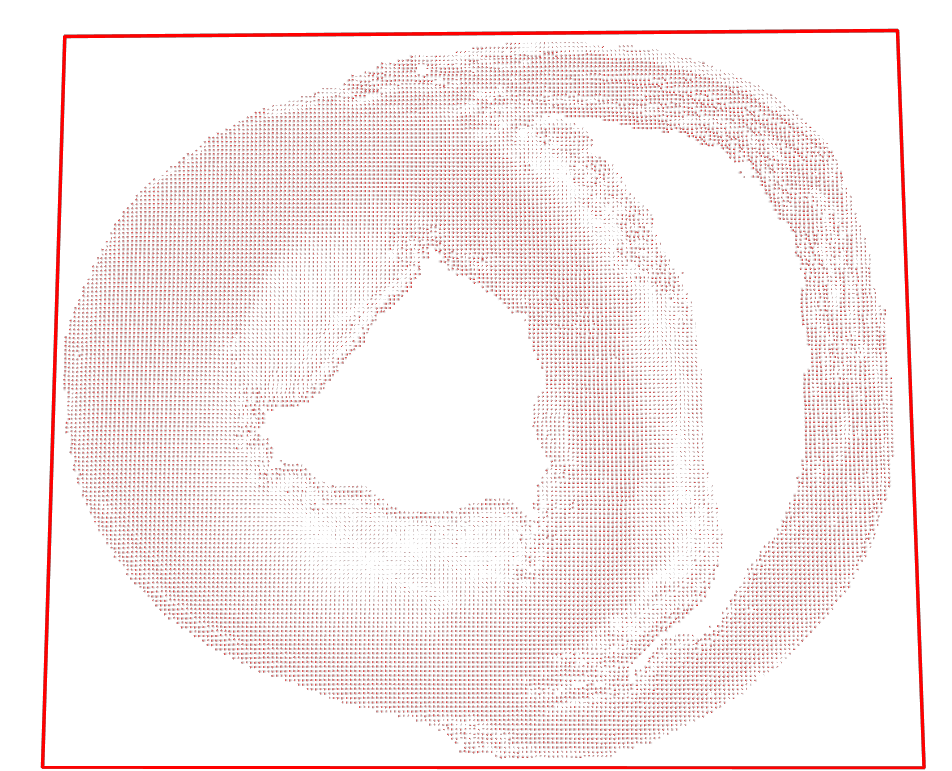
\includegraphics[width=\textwidth]{figures/pig4_topview_smooth}
        \caption{With Rician smoothing}
        \label{fig:pig4_topview_smooth}
    \end{subfigure}
    \caption{Top view of heart fibers for pig 4}
    \label{fig:pig4_topviews}
\end{figure}

\begin{figure}
    \centering
    \begin{subfigure}{.48\textwidth}
        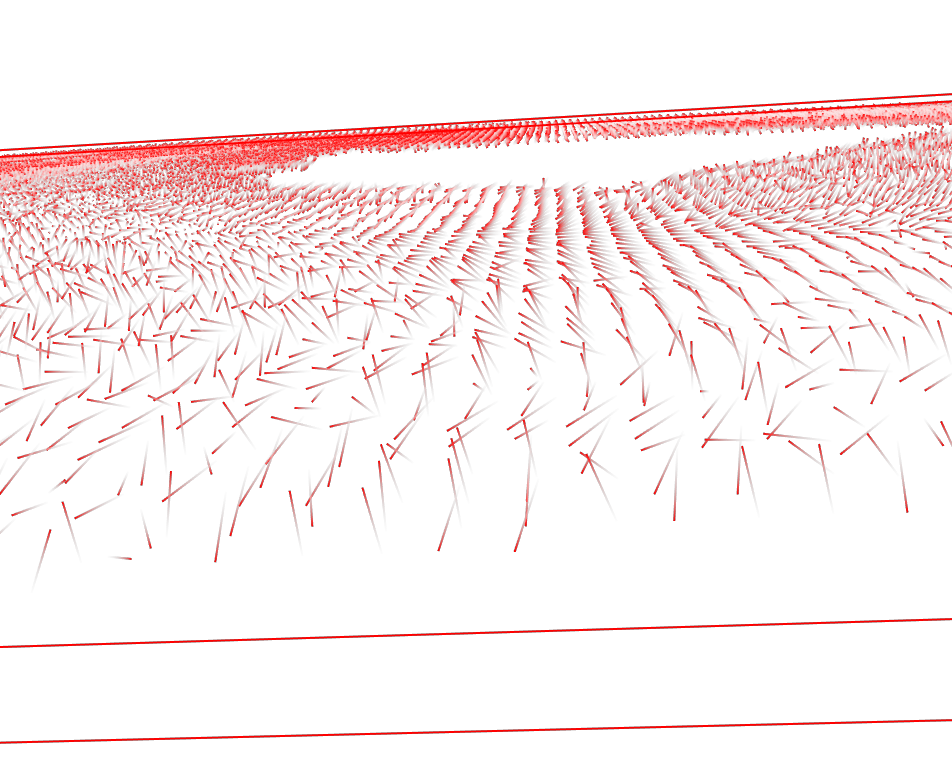
\includegraphics[width=\textwidth]{figures/pig4_helix_no_smooth}
        \caption{Without any smoothing}
        \label{fig:pig4_helix_no_smooth}
    \end{subfigure}
    \begin{subfigure}{.48\textwidth}
        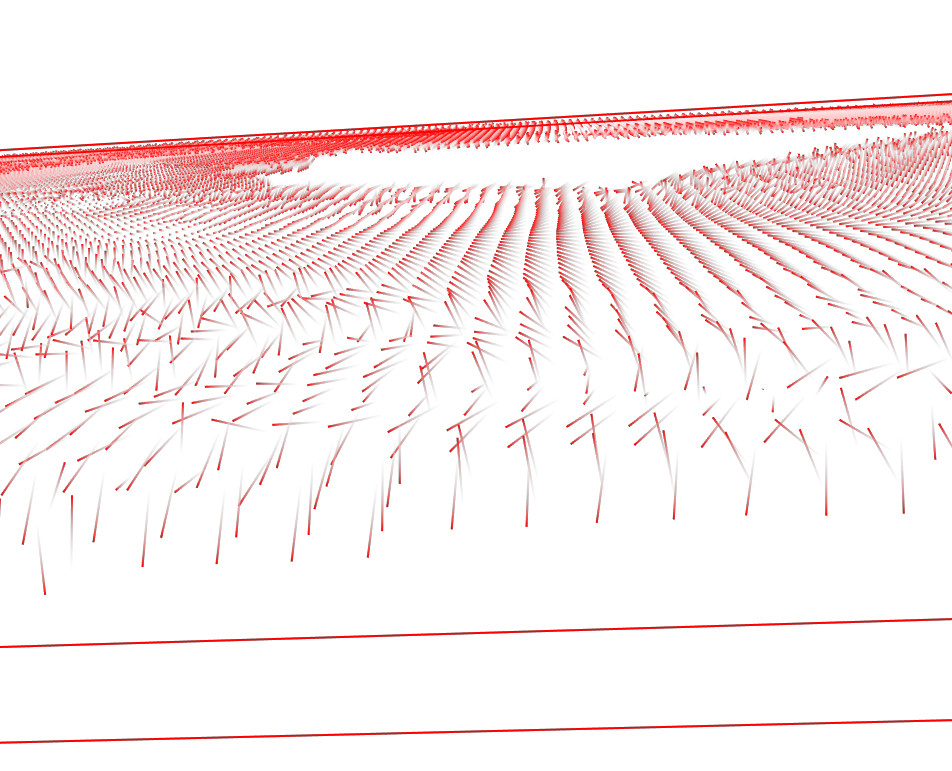
\includegraphics[width=\textwidth]{figures/pig4_helix_smooth}
        \caption{With Rician smoothing}
        \label{fig:pig4_helix_smooth}
    \end{subfigure}
    \caption{View of the helix angle of heart fibers for pig 4}
    \label{fig:pig4_helix}
\end{figure}

\subsection{...To the tractography and fitting process}

Using the fiber orientation that we can get from the computed tensor matrix, we can run tractography on our results. This process gives us an idea of how fibers should be wrapped around the heart and work together in the muscle structure. Looking at the tractography run on the raw data \ref{fig:pig4_tracto_no_smooth} it is hard to see where the infarct would be by just looking at the tracing of existing fibers and trying to infer their direction. The infarct region, as explained in \cite{wu2007mr}, should be the region with the least coherence in its fiber directions whereas regions remote from the infarct should not be affected in their structure.\\
Looking at the tractography run on the Rician smoothed data \ref{fig:pig4_tracto_smooth} on the other hand gives a clear hint on the region where the infarct is present (LAD) whereas remote regions do not seem affected by this and wrap smoothly around the heart.\\
Finally, looking at histograms \ref{fig:pig6_histograms} we can get from our procedure to look at statistics on the visualized information presented, we see several clear indications that smoothing will be a capital step in our further analysis of our datasets:
\begin{enumerate}
    \item Shape of Gaussians we get from the datasets. The center is much better defined in for the smoothed data \ref{fig:histogram_pig6_smooth} as well as overall shape which is less spiky
    \item The number of voxels that count in our computations: from $1564$ with raw unfiltered data \ref{fig:histogram_pig6_no_smooth} to $59187$ after the Rician filter \ref{fig:histogram_pig6_smooth}
\end{enumerate}
The number of voxels that count in our computations is the number of voxels where we could converge to a value of connection form matrix $(c_{i, j, k})_{(i, j, k) \in \mathbb{R}^3}$. Voxels where we could not converge to a value after a given number of iterations were discarded in the histogram to limit the noise importance in the final observations.

\begin{figure}
    \centering
    \begin{subfigure}{.48\textwidth}
        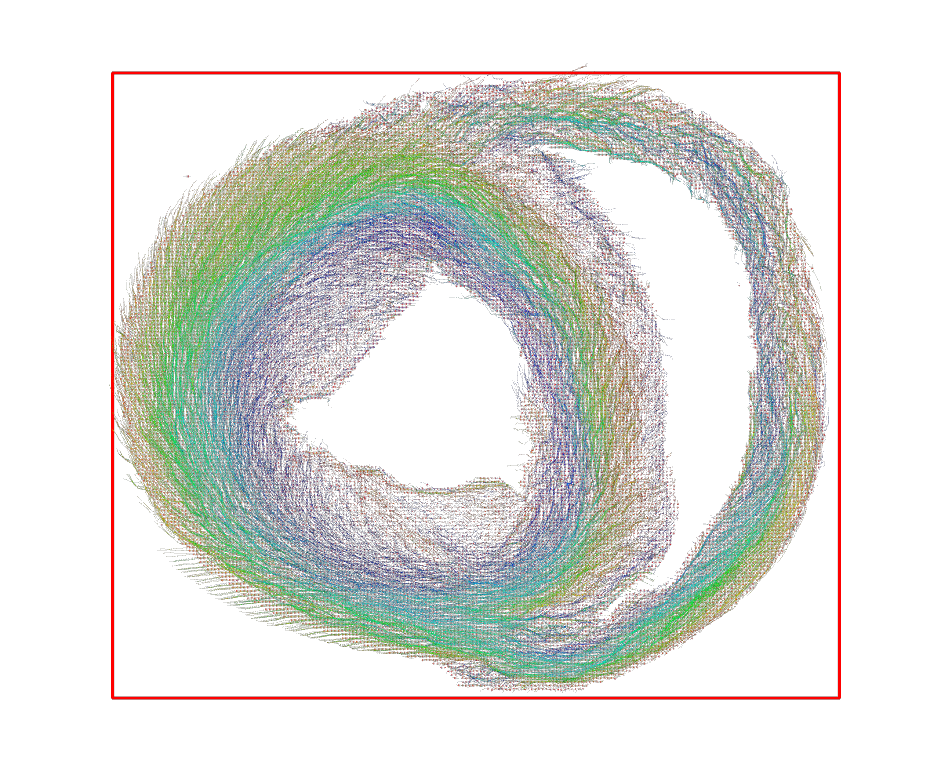
\includegraphics[width=\textwidth]{figures/pig4_topview_tracto_no_smooth}
        \caption{Without any smoothing}
        \label{fig:pig4_tracto_no_smooth}
    \end{subfigure}
    \begin{subfigure}{.48\textwidth}
        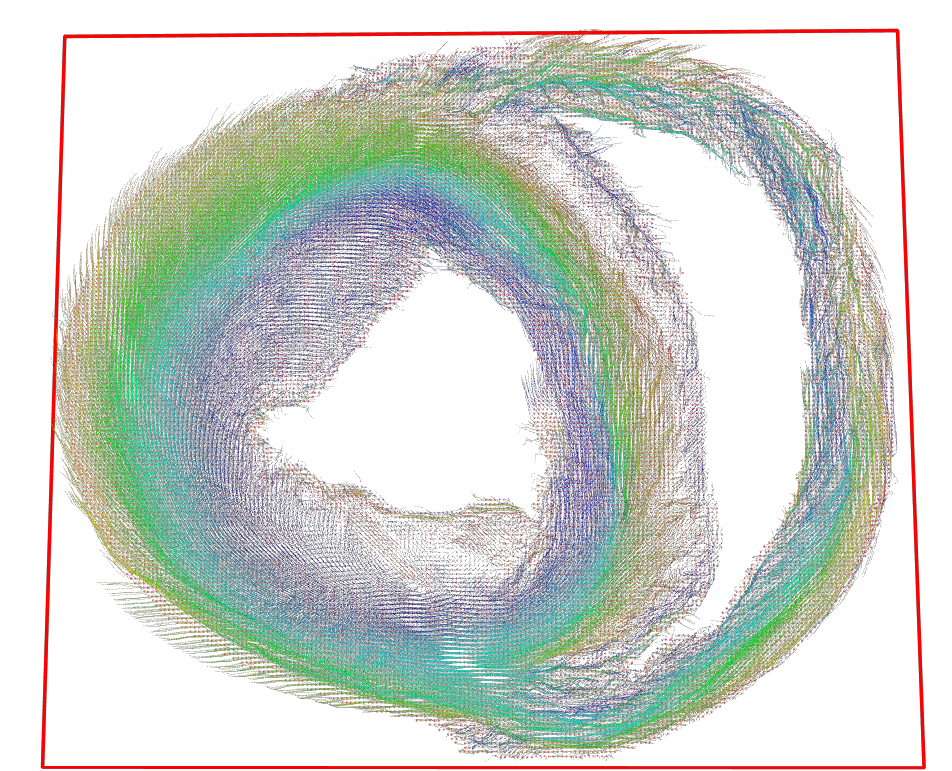
\includegraphics[width=\textwidth]{figures/pig4_topview_tracto_smooth}
        \caption{With Rician smoothing}
        \label{fig:pig4_tracto_smooth}
    \end{subfigure}
    \caption{Tractography of heart fibers for pig 4}
    \label{fig:pig4_tractos}
\end{figure}

\begin{figure}
    \centering
    \begin{subfigure}{.48\textwidth}
        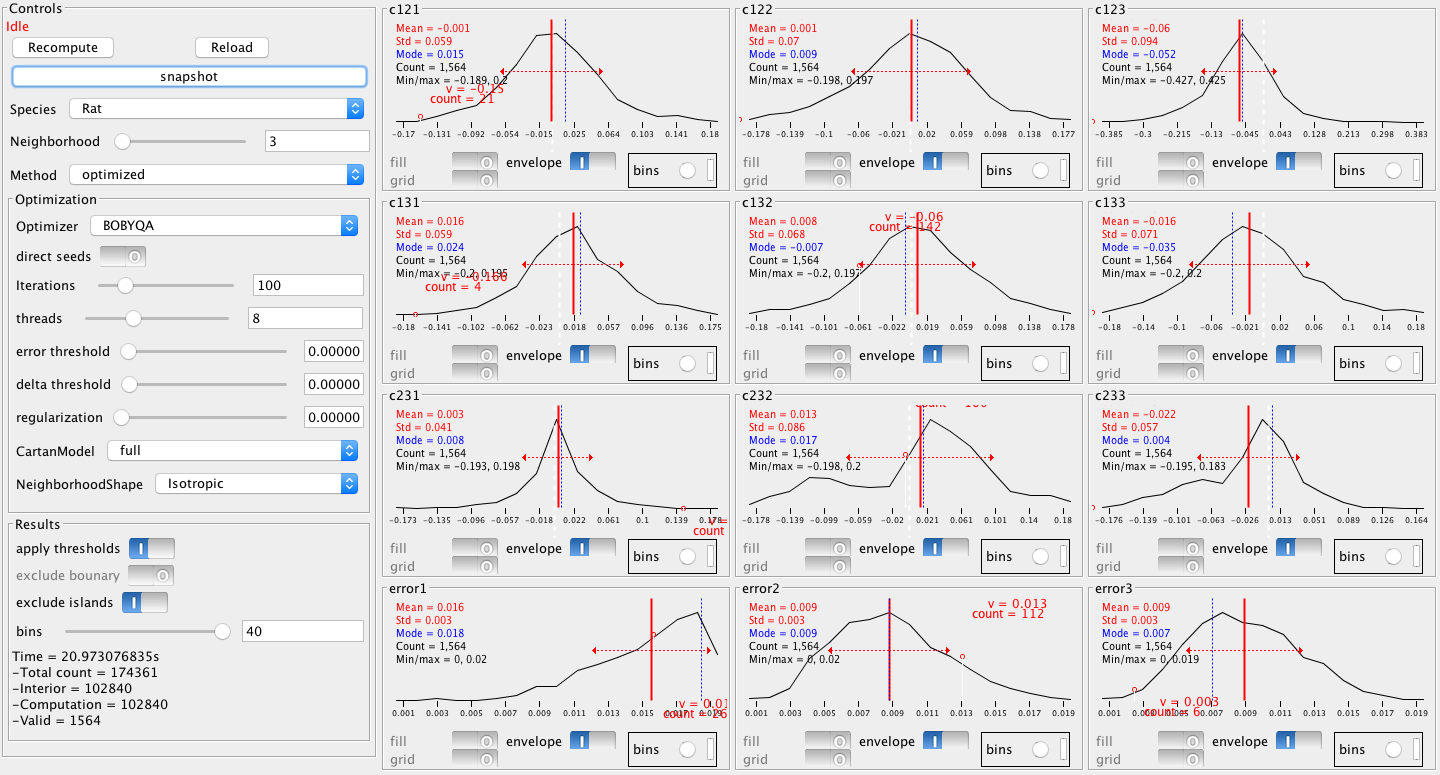
\includegraphics[width=\textwidth]{figures/histogram_pig6_no_smooth}
        \caption{Without any smoothing}
        \label{fig:histogram_pig6_no_smooth}
    \end{subfigure}
    \begin{subfigure}{.48\textwidth}
        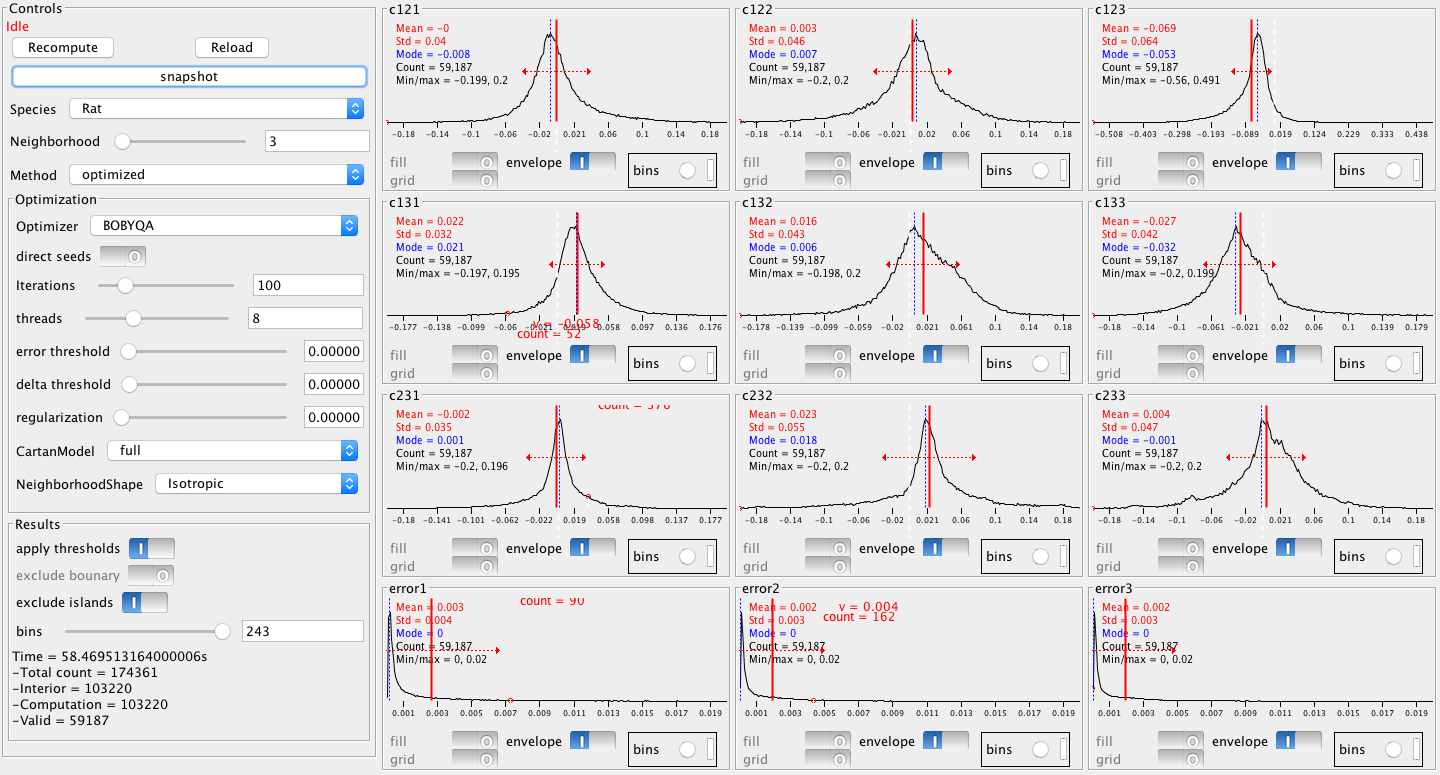
\includegraphics[width=\textwidth]{figures/histogram_pig6_smooth}
        \caption{With Rician smoothing}
        \label{fig:histogram_pig6_smooth}
    \end{subfigure}
    \caption{Histogram of model fitting on raw and smoothed data}
    \label{fig:pig6_histograms}
\end{figure}

\subsection{Discussion}

Supplementing the earlier results in Fig. 1, Fig 3 compares ADC maps (top row) with our Cartan frame fitting-based error of fit maps in degrees (second row) for a healthy pig heart (left column) and 2 additional infarcted hearts (middle and right columns). In all these examples locations where the ADC value is high are typically also ones where the error of fit is high, with regions of low error of fit being restricted to healthy tissue. In addition though, the error of fit is also consistently high at locations close to the epithelial and endothelial boundaries, signaling a loss in geometric coherence of fibers there. Curiously this phenomena is also seen at the borders of the healthy heart (Fig. 3 left column).

\section{Quantitative Results}

Given the association between ADC and our error of frame fit, it is natural to compare these measures quantitatively throughout the myocardium. We did so for the 5 infarcted porcine hearts we analyzed by computing Dice coefficients to describe the overlap, in the following manner. For the same heart let A be the set of voxels with ADC value > 0.6 and let B be the set of voxels with error of fit > 15 degrees. We computed the standard Dice coefficient A∩B/A∪B as well as a modified coefficient A∩B/A. These results, shown in Table. 1 (left), demonstrate that typically over 80\% of the locations with increased diffusion also yield a high error of fit using our frame fitting method, due to the loss of geometric coherence of fiber orientations. However there are additional locations where fiber orientations are not smooth, typically at the linings of the heart wall, or near the edges of a collapsing and narrow right ventricle. These